%%
%% Capítulo 4: Figuras, gráficos e tabelas
%%

\mychapter{Experimentos e Resultados}
\label{Cap:ExperimentosResultados}
Neste trabalho foram feitos dois experimentos em relação a criação
de um modelo cinemático para o robô, o primeiro experimento foi o
treinamento de um modelo de rede neural simples, onde o algoritmo
de aprendizado supervisionado deve buscar uma transformação linear,
que mapeia velocidade linear e angular do robô para as velocidades
angulares das rodas sem levar em consideração as equações das rodas,
o segundo experimento é o treinamento de um modelo cujo os parâmetros
são constantes das equações rodas, onde o algoritmo de aprendizado
de máquina deve realizar uma regressão não linear para encontrar
estes parâmetros, por fim é resolvida analaticamente a cinemática
com a finalidade de comparar com os dois modelos. Em relação ao controlador,
foi implementado o controlador Vieira e encontradas as constantes do P.I.D
empiricamente.


\section{Experimentos com a Cinemática}
Em todos os treinamentos dos modelos
de rede neural artificial foi utilizado o algoritmo de otimização
RMSprop com uma taxa de aprendizado de 0,0001, um momentum $m =0$,
foi utilizado o \textit{Framework pytorch}, para a criação dos
grafos computacionais e treinamento dos modelos. \textit{Pytorch}
permite a criação e prototipagem de um modelo de aprendizagem de
máquina na linguagem \textit{Python} ao mesmo tempo que possui
uma versão em C++ e \textit{Rust}, permitindo criar aplicações
bastante performáticas. Em nosso Experimentos a execução do modelo
em \textit{Rust} é em média 2 vezes mais rápido do que a mesma implementação
em \textit{Python}, para se chegar a esse número foi executado 10 mil vezes o cálculo
da cinemática, em um \textit{notebook} com processador de 4 núcleos \textit{AMD Ryzen 5 2500U},
sem placa de vídeo dedicada. Para a criação dos modelos foi executado o
algoritmo de coleta de dados obtendo conjunto com 10 mil
pontos. Durante o treinamento é dividido este conjunto de dados
onde 60\% dos dados são utilizados para treinamento e 40\% foi utilizado
apenas para avaliação, ou seja, a rede não possui informação sobre esses
pontos durante o treinamento, nas figuras \ref{fig:error:quadratico:nao:linear} e
\ref{fig:error:quadratico:linear} a linha vermelha representa o erro de
Avaliação, e a linha azul representa o erro durante o treinamento,
a métrica de erro utilizada para o treinamento e avaliação
foi o erro quadrático médio.

\begin{figure}[H]
    \label{fig:error:quadratico:nao:linear}
    \centering
    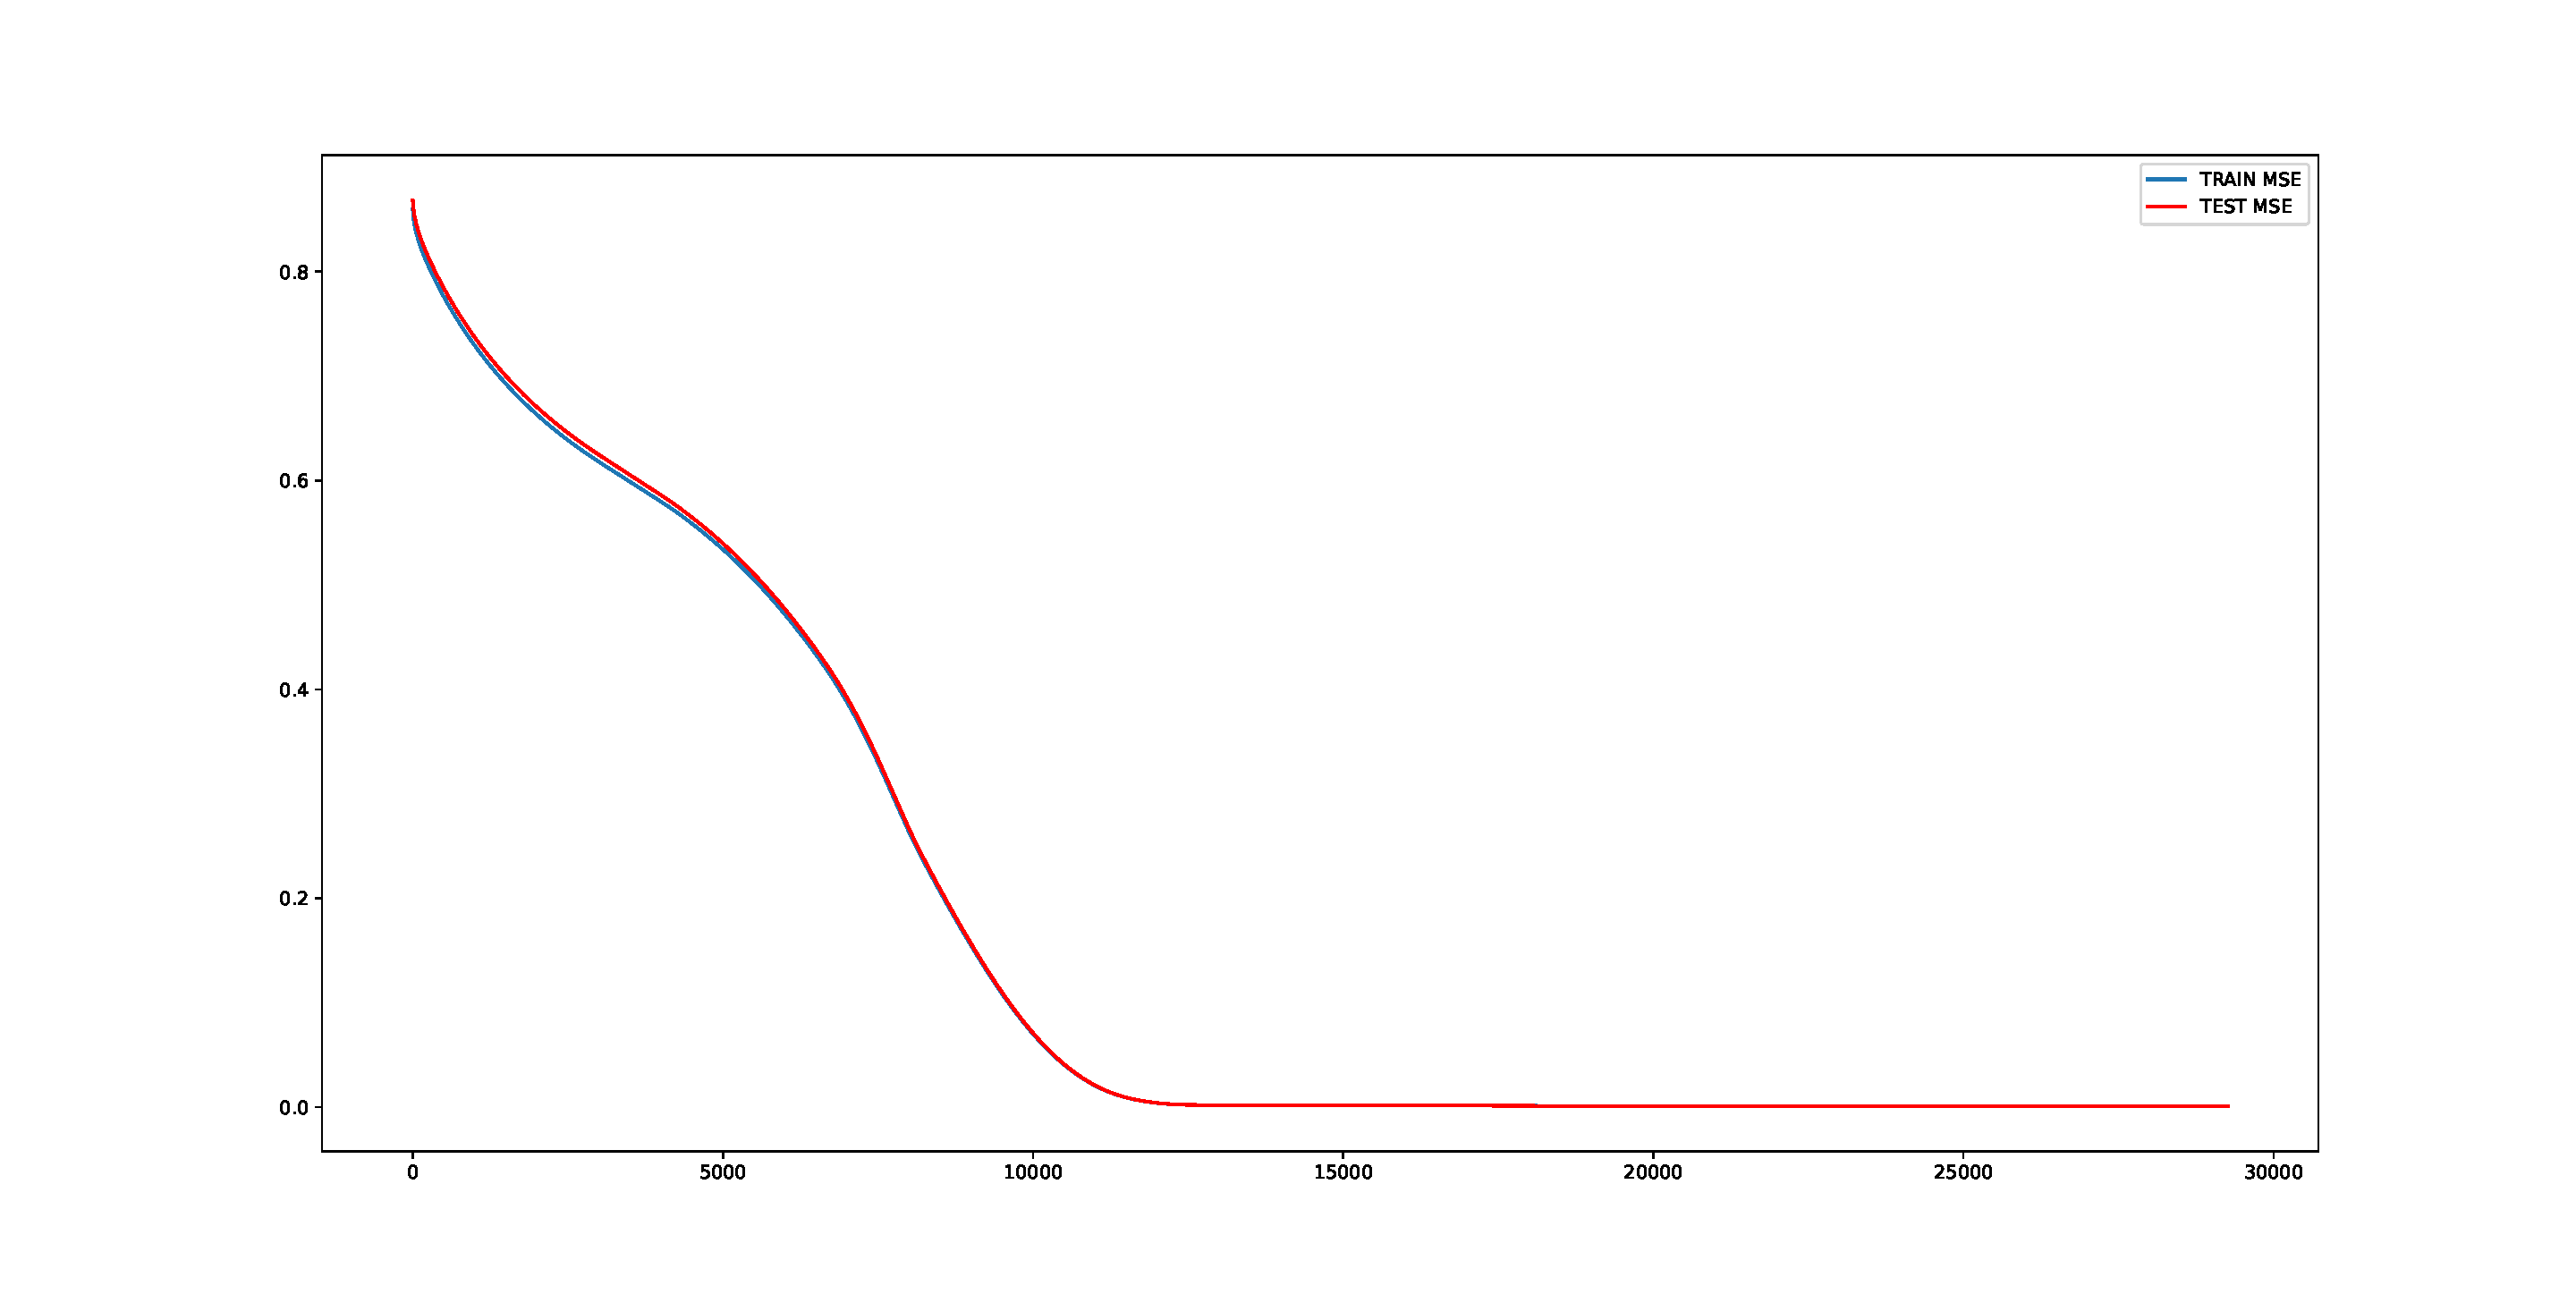
\includegraphics[scale=0.3]{figuras/MSE_error_non_linear.pdf}
    \caption{Erro Médio quadrático regressão não linear}
\end{figure}

\begin{figure}[H]
    \label{fig:error:quadratico:linear}
    \centering
    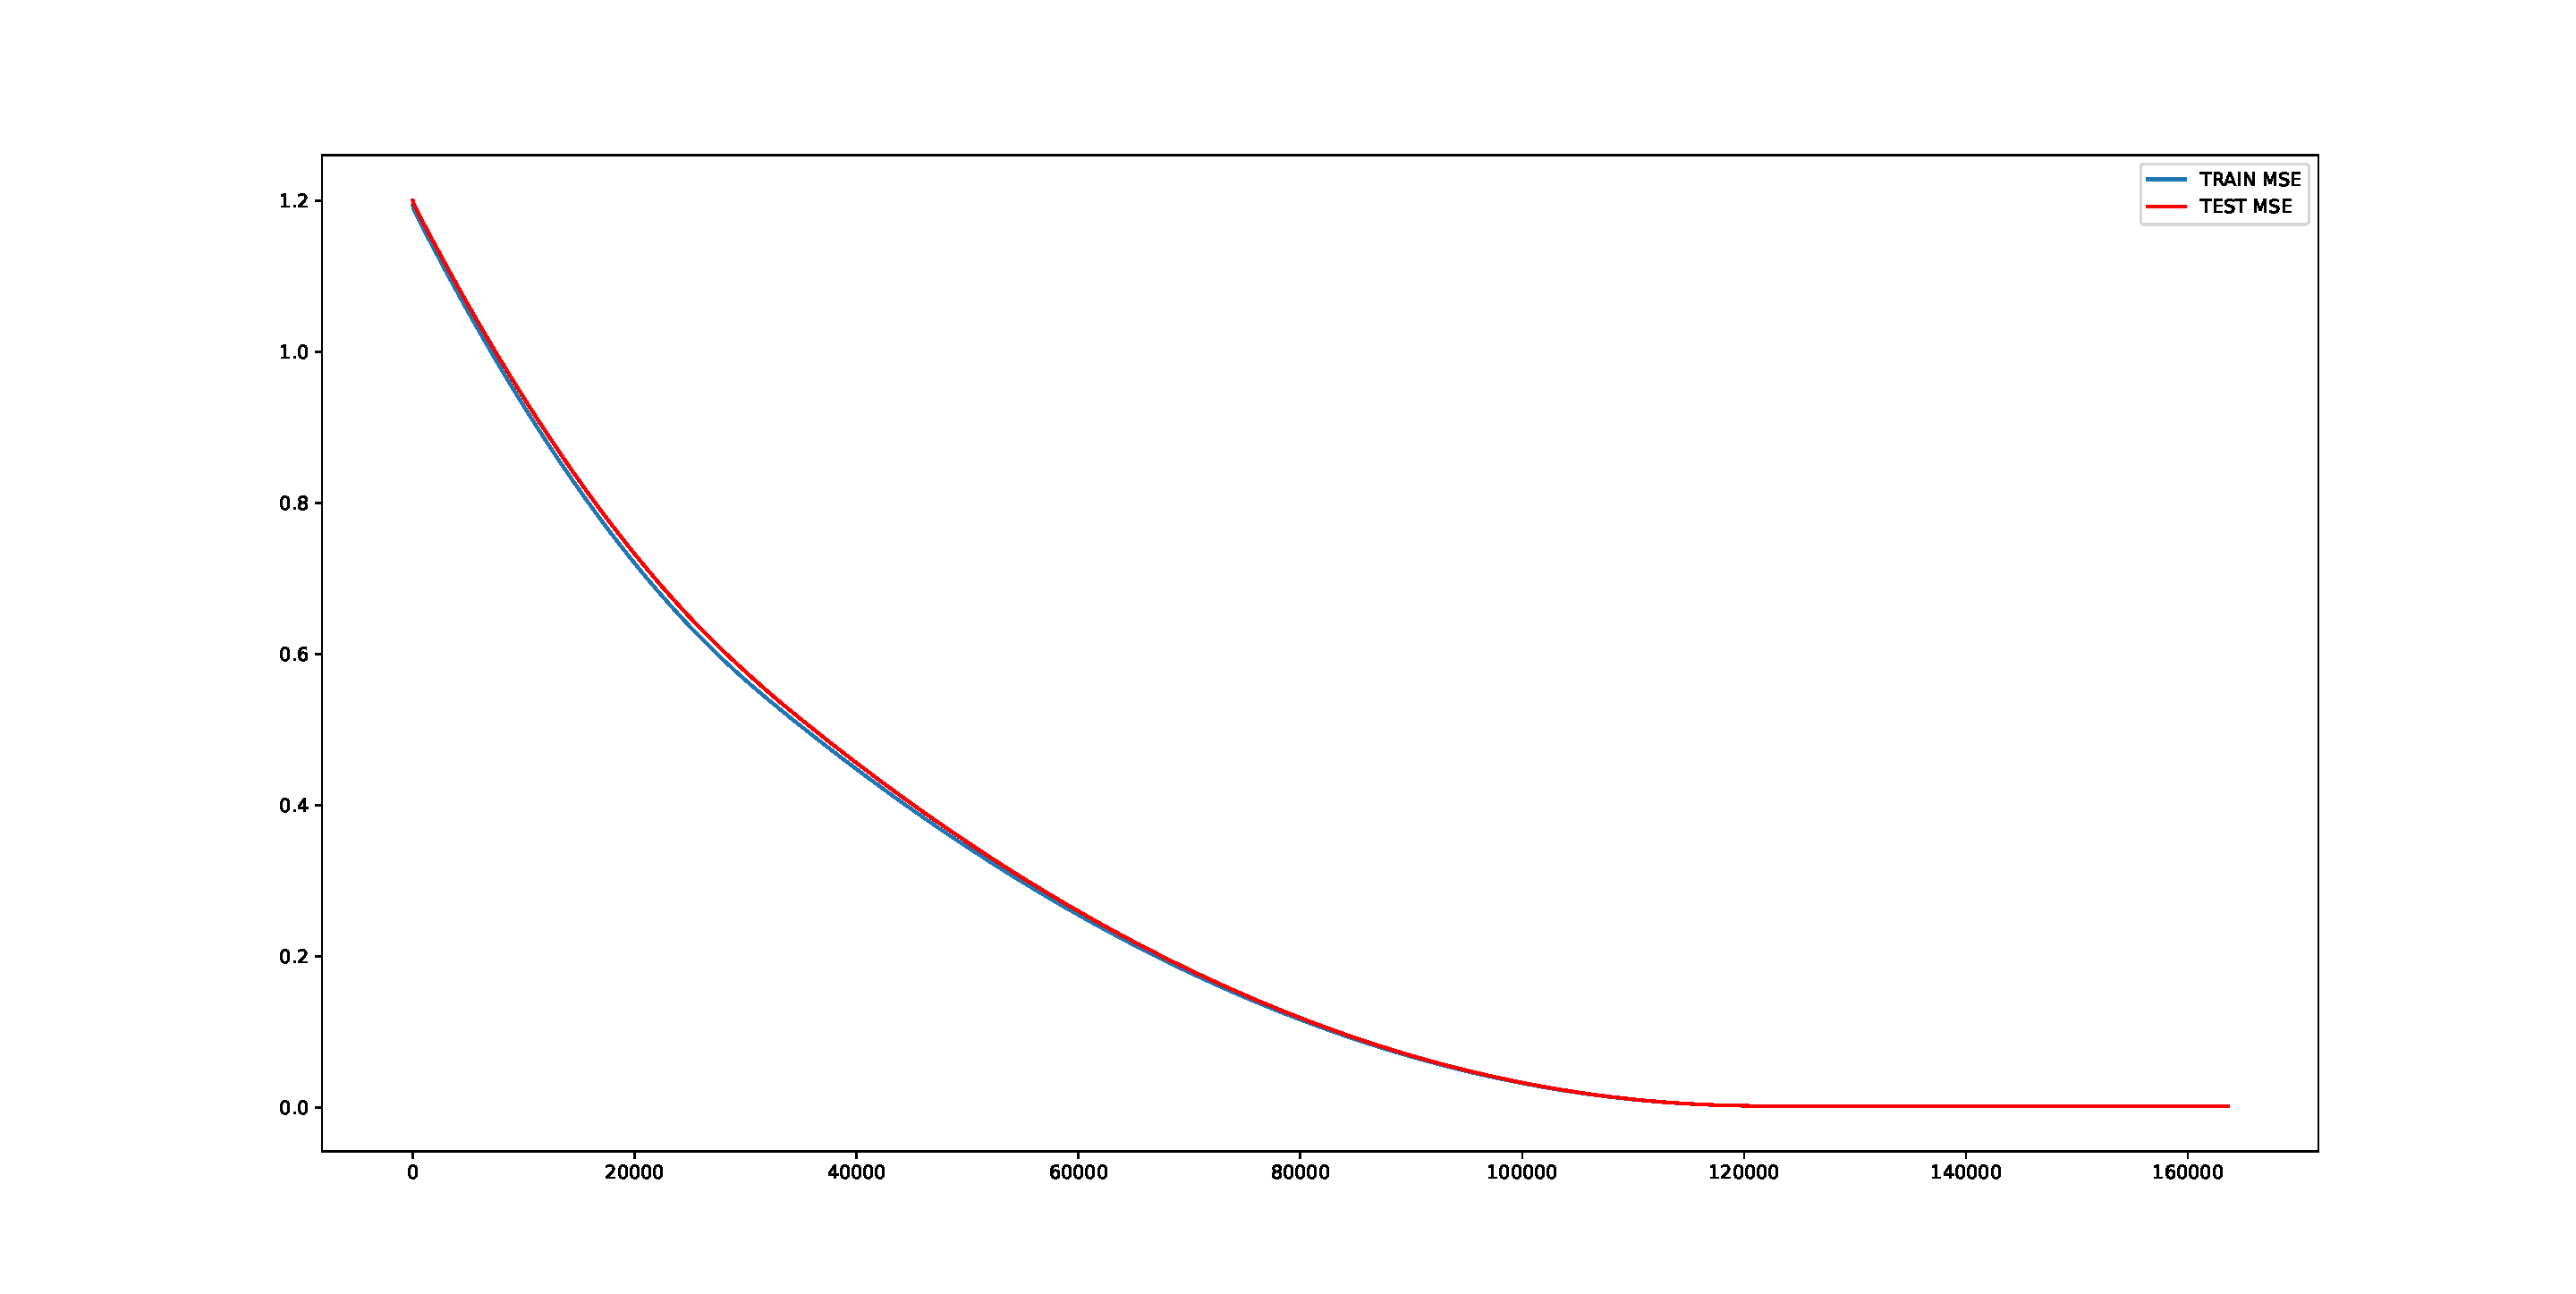
\includegraphics[scale=0.3]{figuras/mse_error_linear.pdf}
    \caption{Erro Médio quadrático regressão linear}
\end{figure}

Para teste dos modelos cinemáticos foram coletados mais 10 mil pontos,
mas dessa vez com o robô podendo variar a velocidade angular das rodas
para até 5 vezes o raio da roda, ou seja $V_{MAX}=5$, no entanto ao invés
de coletar dados de posição, foi extraído do simulador diretamente a
velocidade do robô.

\begin{figure}[H]
    \label{fig:conj:dados}
    \centering
    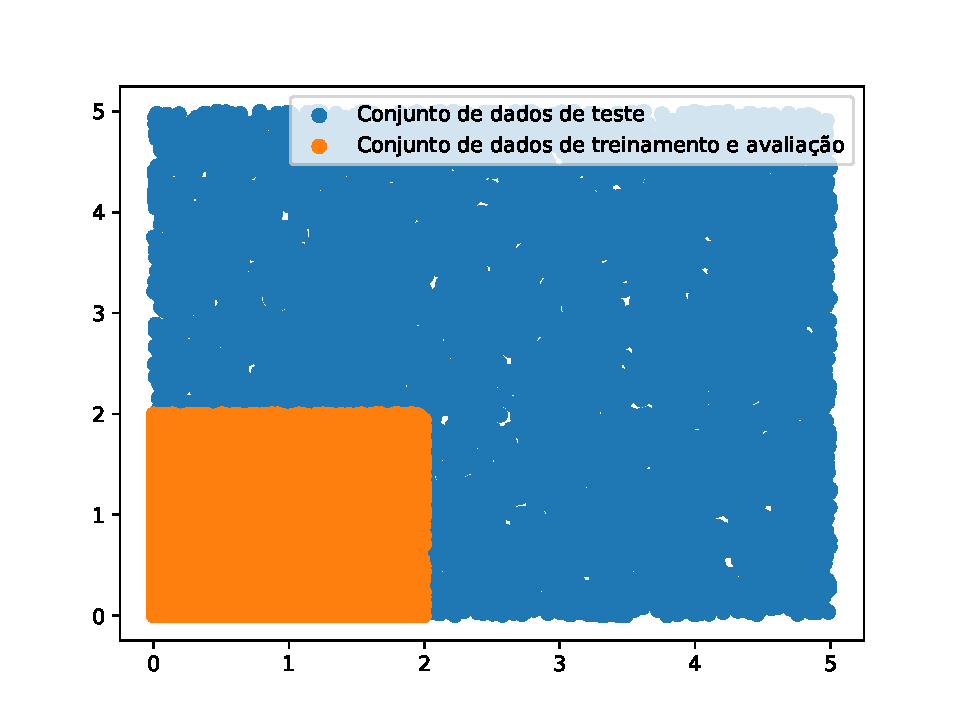
\includegraphics[scale=0.5]{figuras/conj_dados.pdf}
    \caption{Comparação entre os conjuntos de dados}
\end{figure}

Podemos observar que na figura \ref{fig:conj:dados} que o conjunto
de dados para treinamento e avaliação do modelo 
é um sub conjunto do conjunto de testes. Foi calculado o erro quadrático
médio dos modelos em relação ao conjunto de testes gerando a
tabela \ref{table:mse:test}


\begin{table}[H]
    \label{table:mse:test}
    \centering
    \begin{tabular}{c|c}
        \hline
        Erro quadrático médio & modelo \\
        \hline
        0,0037 & modelo regressão linear \\
        \hline
        0,0032 & modelo regressão não linear \\
        \hline
        0,0027 & modelo analítico \\
        \hline
    \end{tabular}
    \caption{teste dos modelos}
\end{table}

Como se sabe o significado físico dos parâmetros do modelos gerados
através de algoritmos de aprendizado de máquina, então na figura
\ref{fig:parametros:da:cinemantica} mostra os valores encontrados
sendo $W_{A}$ os valores do calculo analítico, $W_{K}$ e $W_{L}$ 
são os valores obtidos através da regressão não linear e linear
respectivamente. A tabela \ref{table:param:kinematic} mostra os valores
dos parâmetros das rodas após a regressão não linear, e a tabela
\ref{table:param:analytic} mostra os valores dos parâmetros da
solução analítica, em ambas as tabelas os ângulos estão medidos
em graus, e os raio da roda $r$ e distância $l$ estão em metros.
 
\begin{figure}[H]
    \label{fig:parametros:da:cinemantica}
    \begin{align*}
        W_{A} = 
        \begin{bmatrix}
            12,1212 &  0,0000 & 3,5307 \\
            12,1212 &  0,0000 & -3,5307 \\
        \end{bmatrix}\\
        W_{K} = 
        \begin{bmatrix}
            12,2294 &  -0,0291 & 3,7330 \\
            12,1241 &  -0,1347 & -3,5121
        \end{bmatrix}\\
        W_{L} = 
        \begin{bmatrix}
            12.2262 &  -1.3070 & 3.5472 \\
            12.1198 &  -4.4313 & -4.1472
        \end{bmatrix}\\
    \end{align*}
    \caption{Modelos cinemáticos}
\end{figure}

\begin{table}[H]
    \label{table:param:kinematic}
    \centering
    \begin{tabular}{c|c|c|c|c}
        \hline
         $\alpha$ &$\beta$ &$l$ &$r$ & roda \\
        \hline
        115,6515 &-25,8002 &-0,3389 &0,0818 & roda esquerda \\
        \hline
        62,3091  &27,1352 &0,3254 &0,0825 & roda direita \\
        \hline
    \end{tabular}
    \caption{parâmetros das rodas após a regressão não linear}
\end{table}
Perceba que o angulo $\gamma = \alpha + \beta$ do modelo gerado pela regressão não
linear foi de $\gamma_{k_1} = 115,6515 -25,8002  = 89,8513$ e 
$\gamma_{k_2} = 62,3091 +27,1352 = 89,4443$
\begin{table}[H]
    \label{table:param:analytic}
    \centering
    \begin{tabular}{c|c|c|c|c}
        \hline
         $\alpha$ &$\beta$ &$l$ &$r$ & roda \\
        \hline
        90 & 0 &-0,2912 &0,0825 & roda esquerda \\
        \hline
        -90  & 180 & 0,2912 &0,0825 & roda direita \\
        \hline
    \end{tabular}
    \caption{parâmetros das rodas modelo analítico}
\end{table}


Como dito anteriormente foi utilizado o controlador Vieira,
cujo os parâmetros dos P.I.Ds foram adquiridos empiricamente,
visando minimizar o sobre-sinal do controlador de velocidade linear,
os valores podem ser vistos na tabela \ref{table:pid:}.

\begin{table}[H]
    \label{table:pid:}
    \centering
    \begin{tabular}{c|c|c|c}
        \hline
        P & I & D & tipo de controlador \\
        \hline
        0,05145 & 0,01769 & 0,60529 & velocidade linear \\
        \hline
        0,4 & 0,015 & 0 & velocidade angular \\
        \hline
    \end{tabular}
    \caption{parâmetros P.I.D}
\end{table}

Para avaliar o sistema de controle, com os diferentes modelos
cinemáticos, foi posicionado um alvo e observado o robô no seu
trabalho em chegar até alvo mensurando a distância e o angulo do robô até
o alvo, essas duas medidas foram escolhidas pois 
estes são os valores a serem minimizados pelo controlador Vieira,
o alvo foi posicionado em quatro lugares diferentes como mostra a figura
\ref{fig:robo:e:4:alvos}.

\begin{figure}[H]
    \label{fig:robo:e:4:alvos}
    \centering
    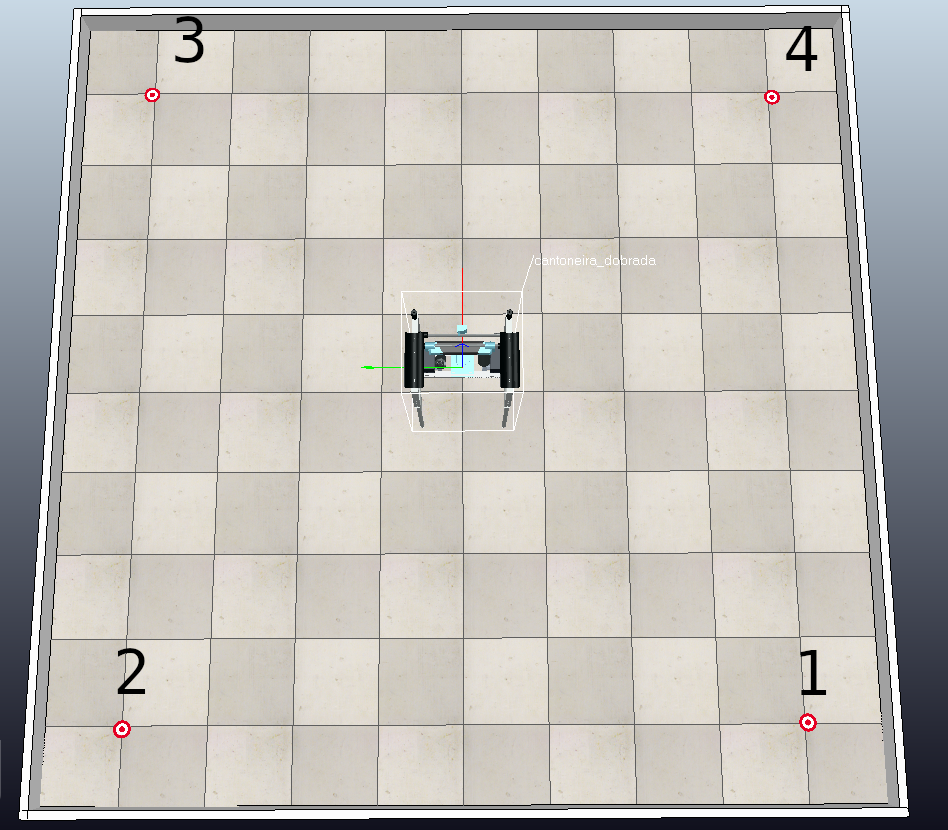
\includegraphics[scale=0.3]{figuras/robo_e_alvo.png}
    \caption{Robô e alvo}
\end{figure}

\begin{figure}[H]
    \centering
    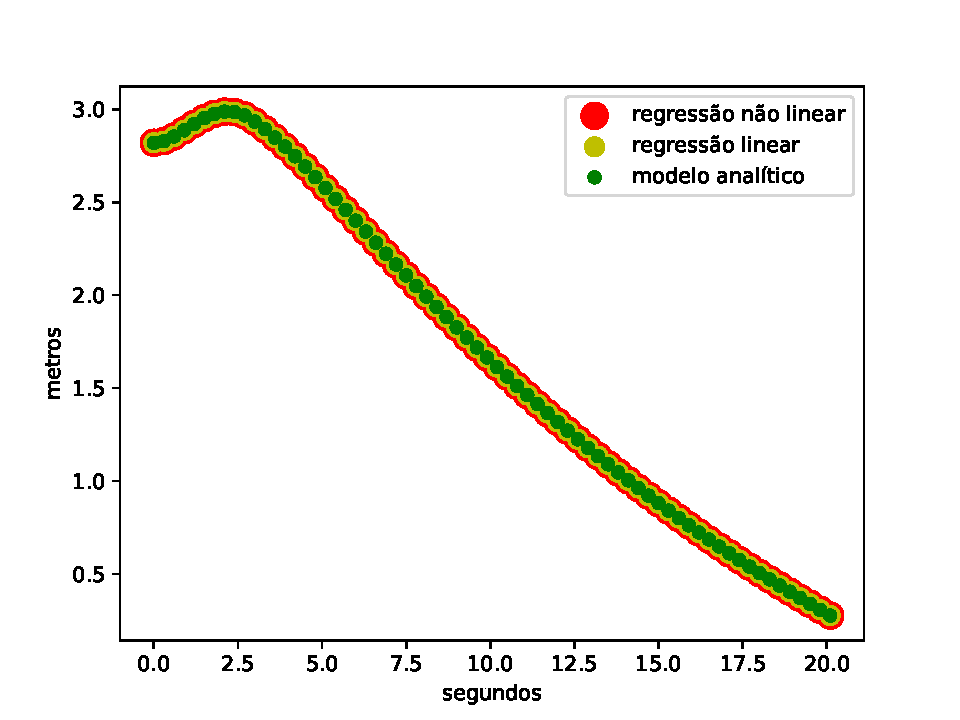
\includegraphics[scale=0.45]{figuras/distance_over_time_1.pdf}
    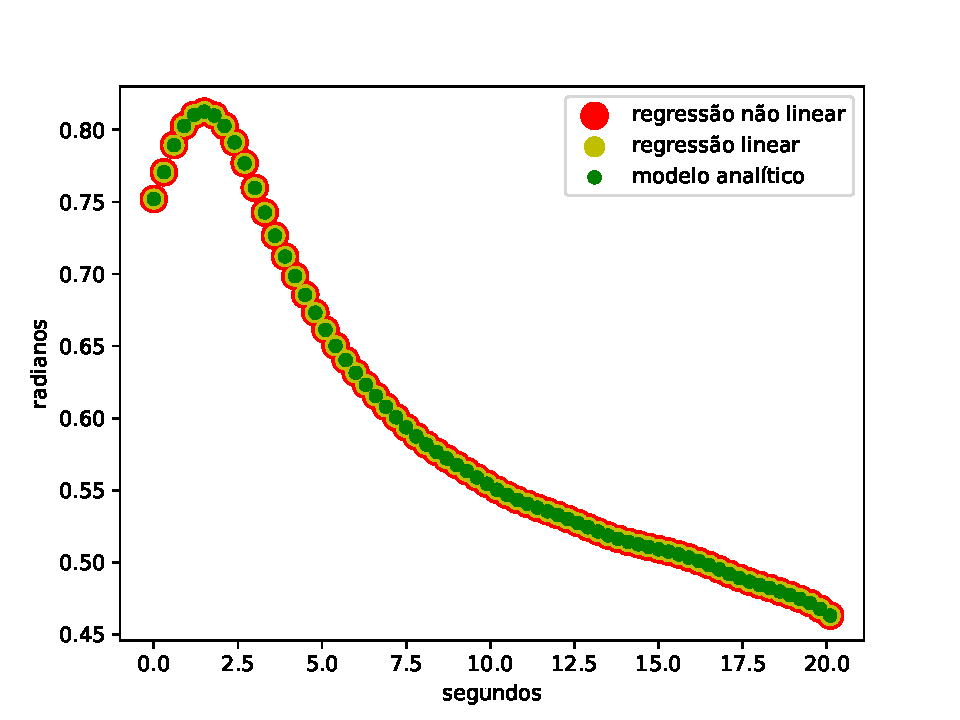
\includegraphics[scale=0.45]{figuras/angle_over_time_1.pdf}
    \caption{Angulo e distância observada no alvo 1}
\end{figure}

\begin{figure}[H]
    \centering
    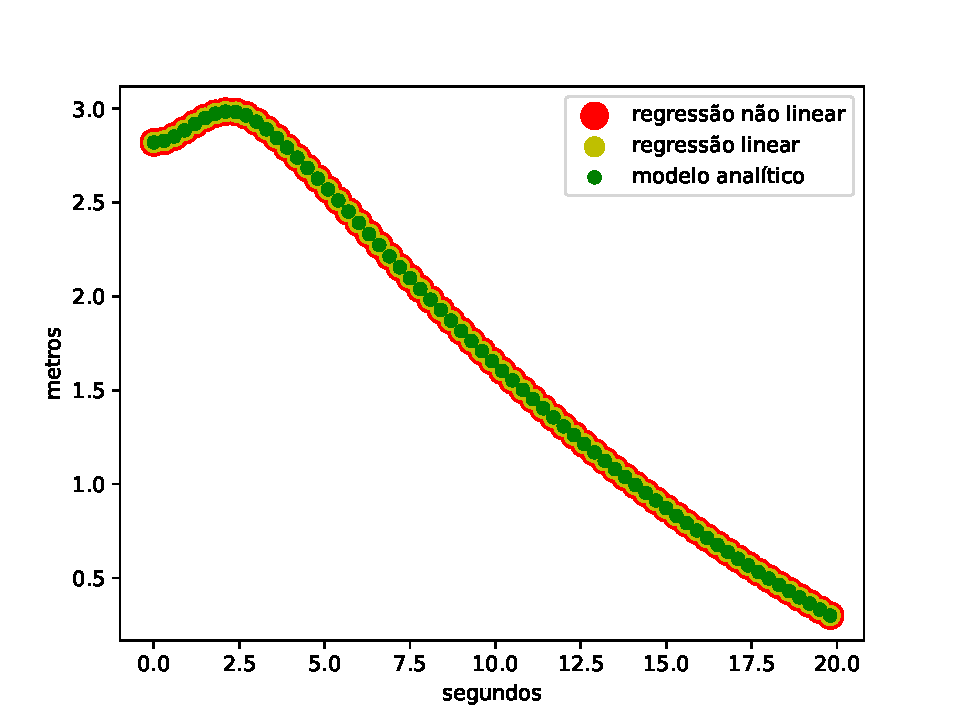
\includegraphics[scale=0.45]{figuras/distance_over_time_2.pdf}
    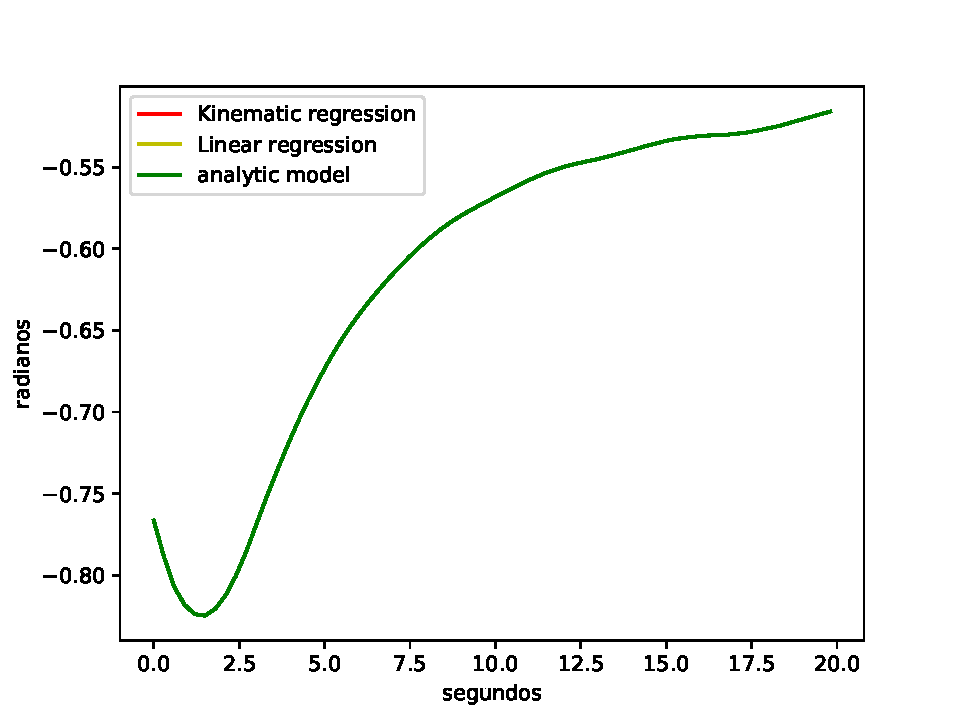
\includegraphics[scale=0.45]{figuras/angle_over_time_2.pdf}
    \caption{Angulo e distância observada no alvo 2}
\end{figure}

\begin{figure}[H]
    \centering
    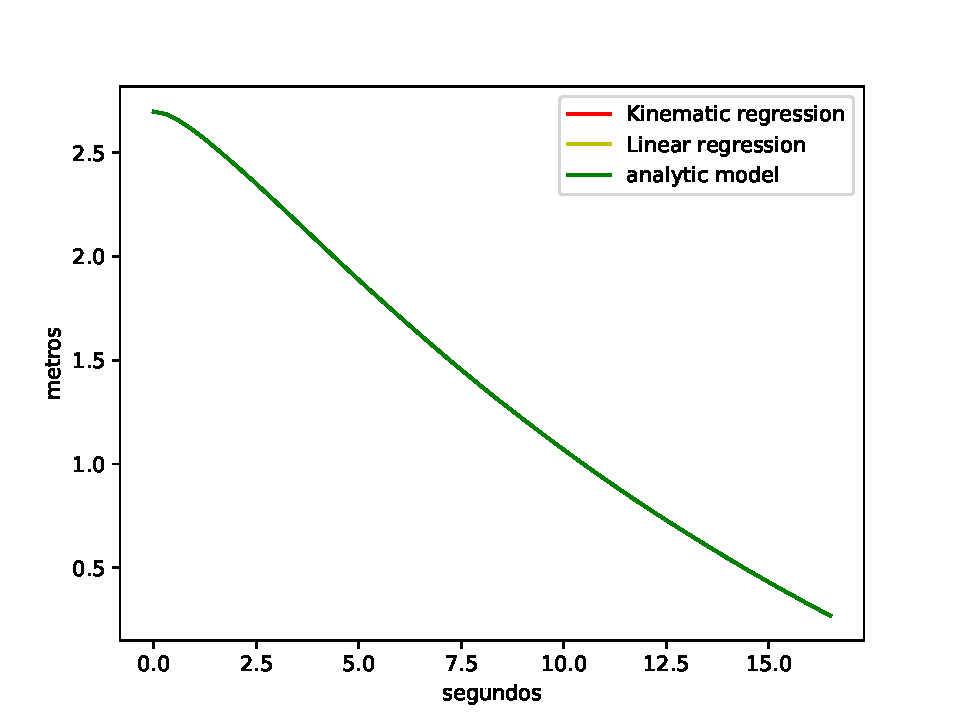
\includegraphics[scale=0.45]{figuras/distance_over_time_3.pdf}
    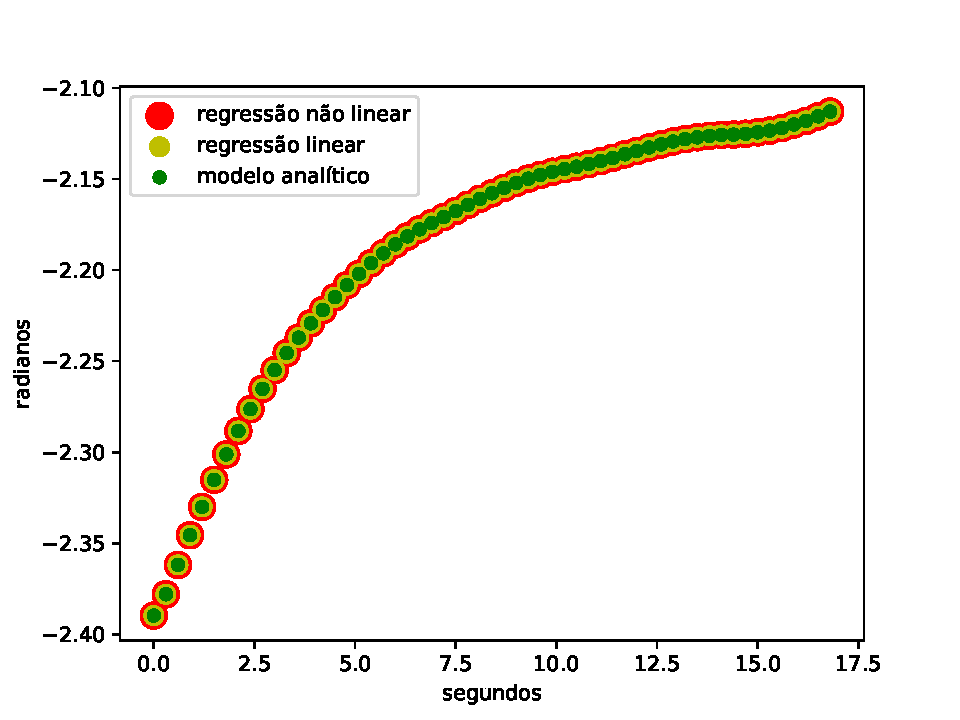
\includegraphics[scale=0.45]{figuras/angle_over_time_3.pdf}
    \caption{Angulo e distância observada no alvo 3}
\end{figure}

\begin{figure}[H]
    \centering
    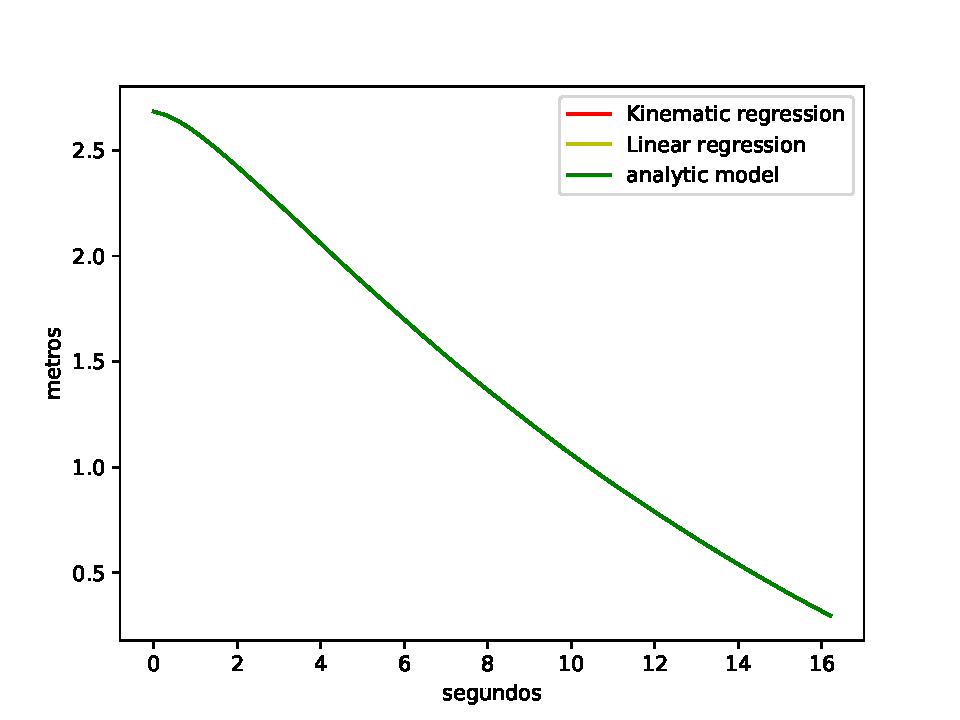
\includegraphics[scale=0.45]{figuras/distance_over_time_4.pdf}
    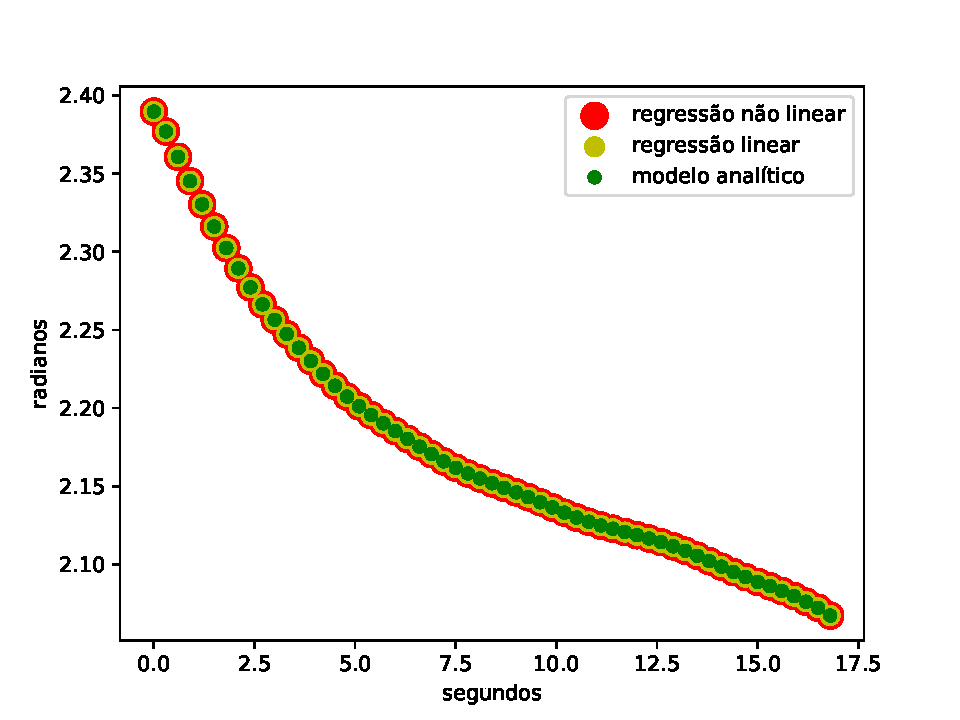
\includegraphics[scale=0.45]{figuras/angle_over_time_4.pdf}
    \caption{Angulo e distância observada no alvo 4}
\end{figure}

Perceba os pontos dos modelos obtidos através da regressão e o modelo analítico
estão sobrepostos. Quando o centro geométrico do robô está a uma distância menor que 30 centímetros
do alvo o sistema de controle entende que o robô chegou na posição desejada.

\section{Discussão dos Experimentos}
Na observação do robô em seu trabalho de chegar até o alvo, os modelos
obtidos através da regressão linear e não linear tiveram respostas
idênticas ao modelo analítico, também na tabela do erro quadrático médio \ref{table:mse:test},
os valores ficaram nas mesmas casas decimais, através desses dois fatos
podemos dizer que os modelos são equivalentes, outro ponto interessante é
observar a generalização do modelos, uma vez que o conjunto do treinamento
é um sub conjunto do conjunto de testes o que nos dá segurança em aplicar
o modelo em dados nunca vistos, em aprendizado de máquina supervisionada
muitas vezes é feita uma escolha em generalização e otimização, onde um
modelo mais otimizado ao conjunto de dados de treinamento tende a não ir
bem e dados fora desse conjunto, no entanto ao modelarmos o sistema cinemático
do robô ao mesmo tempo que modelamos os pesos de uma rede neural artificial,
mostramos que otimizar os parâmetros de uma rede neural modelada estamos
também aumentando a sua generalização.
Comparando os modelos de aprendizado, podemos observar que a regressão
linear durou cento e sessenta mil iterações, já a regressão não linear parou de reduzir
o erro com trinta mil iterações, apesar do tempo de treinamento está
fortemente relacionado om os valores iniciais da rede, a regressão não
linear teve mais duas equações iguais a zero que ajudou a guiar o erro
mais rápido. Outro ponto interessante de se notar na figura \ref{fig:parametros:da:cinemantica}
é que os pesos da regressão linear afirmam existir uma contribuição negativa
de velocidade linear no eixo y do robô, algo também observado no modelado de
regressão não linear, só que com valores inferiores devido as equações,
talvez estes valores deve-se a aproximação da velocidade por meio da variação
de posição sobre variação do tempo ou algum fator dinâmico da simulação.
Comparando os valores das tabelas \ref{table:param:kinematic} e \ref{table:param:analytic}
podemos perceber que a rede convergiu o angulo $\gamma = \alpha + \beta$,
uma vez que o gamma analítico é  $\gamma_{A} = 90$ e o gamma do modelo
de regressão não linear foi de $\gamma_{K} = 89$. O modelo de aprendizado
de máquina é resultado dos seus dados, como existe uma pequena velocidade
no eixo y do robô, a rede reajustou os parâmetros $l$ e $\beta$ de modo que
representa-se os dados, apensar do modelo não ter encontrado os ângulos,
$\beta, \alpha$ próximos da solução analítica, os raios da rodas estão
com valores muito próximos e a distância $l$ está a uma diferença de
centímetros da solução analítica. Este trabalho também buscar uma solução
que pode-se sem implementada em um computador com limitação de
processamento e memória, então se consideramos que o treinamento poder ser
realizado em outro computador, onde o robô enviaria os dados,
por tanto se consideramos só o sistema de controle, o computador apenas
executará o algoritmo do  P.I.D mais a multiplicação de uma matriz da
cinemática que contem 6 elementos, então o computador utilizado não irá precisar de muita memória e processamento,
sendo a parte mais crítica o armazenamento de um buffer durante o algoritmo
da coleta de dados, outro pronto crítico seria o tempo de bateria durante
a coleta de dados, mas considerando que um ciclo de controle esta por volta
de 30 ms, portanto para coletar 10 mil amostras equivale a 300 segundos, ou
seja, 5 minutos.